\section{Stack Allocation}

\begin{frame}
  \tableofcontents[currentsection]
\end{frame}

\begin{frame}
  \frametitle{Stack Allocation}
  \begin{itemize}
    \item Allocate your variables using static allocation
    \item Introduce {\tt stacknew} keyword that for runtime allocation
    \item Take RAM that's left after static allocation
    \item Act as if it were a \emph{stack} (LIFO) of available bytes
    \item Allocation = take top $N$ bytes
  \end{itemize}
  \vskip5mm
  \begin{center}
    \begin{tikzpicture}
      \draw (0,0) rectangle ++(1,2);
      \draw (1,0) rectangle ++(7,2);

      \node[rotate=90] at (0.5,1) {static};
      \node[rotate=90] at (4.5,1) {stack};

      \draw[|-|] (0,-.5) -- ++(8,0) node[midway,below] {RAM};
    \end{tikzpicture}
  \end{center}
\end{frame}

\begin{frame}
  \frametitle{Stack Allocation Usage}
  \begin{itemize}
    \item Let's use the stack for parameters and local variables
    \item Function call:
          \begin{enumerate}
            \item Allocate space for parameters
            \item Allocate space for locals
            \item Execute body
            \item Free space for locals
            \item Free space for parameters
          \end{enumerate}
    \item Each function call gets own stack frame
          \begin{itemize}
            \item $\rightarrow$ makes recursion possible
          \end{itemize}
  \end{itemize}
\end{frame}



\begin{frame}
  \frametitle{Stack Allocation}
  \begin{columns}
    \column{6cm}
    \code[font=\scriptsize,language=c++14,extra keywords={stacknew}]{stack-allocation.cpp}
    \column{2cm}
    \begin{center}
      \begin{tikzpicture}[allocation/.style={-latex,thick,red},scale=.5,remember picture,overlay]
        \coordinate (start) at (-4,6);

        \only<4>{
          \draw[fill=yellow!50] (start) rectangle ++(4,-10);
        }

        \only<2>{
          \codeunderlinex{stack sum global n}
          \draw[allocation] (stack sum global n) -- ++(0,-0.5) -- ++(5,0) -- ($ (start) + (0,-0.5) $);
        }
        \only<2->{
          \draw[fill=red!50] (start) rectangle ++(4,-1);
        }

        \only<3>{
          \codeunderlinex{stack sum global r}
          \draw[allocation] (stack sum global r) -- ++(0,-0.5) -- ++(5,0) -- ($ (start) + (0,-1.5) $);
        }
        \only<3->{
          \draw[fill=red!50] (start) ++(0,-1) rectangle ++(4,-1);
        }

        \only<5>{
          \codeunderlinex{stack input}
        }

        \only<6>{
          \codeunderlinex{stack sum param}
          \draw[allocation] (stack sum param) -- ++(0,-0.5) -- ++(5,0) -- ($ (start) + (0,-2.5) $);
        }
        \only<6-16>{
          \draw[fill=blue!50] (start) ++(0,-2) rectangle ++(4,-1);
        }

        \only<7>{
          \codeunderlinex{stack sum local}
          \draw[allocation] (stack sum local) -- ++(0,-0.5) -- ++(5,0) -- ($ (start) + (0,-3.5) $);
        }
        \only<7-16>{
          \draw[fill=blue!50] (start) ++(0,-3) rectangle ++(4,-1);
        }

        \only<8>{
          \codeunderlinex{stack sum recursion}
        }

        \only<9>{
          \codeunderlinex{stack sum param}
          \draw[allocation] (stack sum param) -- ++(0,-0.5) -- ++(5,0) -- ($ (start) + (0,-4.5) $);
        }
        \only<9-15>{
          \draw[fill=blue!50] (start) ++(0,-4) rectangle ++(4,-1);
        }

        \only<10>{
          \codeunderlinex{stack sum local}
          \draw[allocation] (stack sum local) -- ++(0,-0.5) -- ++(5,0) -- ($ (start) + (0,-5.5) $);
        }
        \only<10-15>{
          \draw[fill=blue!50] (start) ++(0,-5) rectangle ++(4,-1);
        }

        \only<11>{
          \codeunderlinex{stack sum param}
          \draw[allocation] (stack sum param) -- ++(0,-0.5) -- ++(5,0) -- ($ (start) + (0,-6.5) $);
        }
        \only<11-14>{
          \draw[fill=blue!50] (start) ++(0,-6) rectangle ++(4,-1);
        }

        \only<12>{
          \codeunderlinex{stack sum local}
          \draw[allocation] (stack sum local) -- ++(0,-0.5) -- ++(5,0) -- ($ (start) + (0,-7.5) $);
        }
        \only<12-14>{
          \draw[fill=blue!50] (start) ++(0,-7) rectangle ++(4,-1);
        }

        \only<13>{
          \codeunderlinex{stack sum param}
          \draw[allocation] (stack sum param) -- ++(0,-0.5) -- ++(5,0) -- ($ (start) + (0,-8.5) $);
          \codeunderlinex{stack sum local}
          \draw[allocation] (stack sum local) -- ++(0,-0.5) -- ++(5,0) -- ($ (start) + (0,-9.5) $);
          \draw[fill=blue!50] (start) ++(0,-8) rectangle ++(4,-2);
        }

        \draw (start) grid ++(4,-10);
      \end{tikzpicture}
    \end{center}
  \end{columns}
  \vskip2mm
  \begin{overprint}
    \onslide<2-3>
      \begin{center}
        \textbf{At compile time} \\ 
        Compiler assigns memory locations to globals \\
        (static allocation)
      \end{center}

    \onslide<4>
      \begin{center}
        Remaining memory used as stack
      \end{center}

    \onslide<5>
      \begin{center}
        \textbf{At runtime} \\ 
        Say user enters 3
      \end{center}

    \onslide<6>
      \begin{center}
        \textbf{At runtime} \\ 
        \texttt{sum} gets called with \texttt{n=3} \\
        Parameter \texttt{n} gets its own spot on the stack
      \end{center}

    \onslide<7>
      \begin{center}
        \textbf{At runtime} \\ 
        Local variable \texttt{r} also gets stack space \\
        The function's body execution starts
      \end{center}

    \onslide<8>
      \begin{center}
        \textbf{At runtime} \\ 
        \texttt{sum} gets called recursively
      \end{center}

    \onslide<9>
      \begin{center}
        \textbf{At runtime} \\ 
        A second instance of \texttt{n} equal to \texttt{2} gets pushed onto the stack
      \end{center}

    \onslide<10>
      \begin{center}
        \textbf{At runtime} \\ 
        A second instance of \texttt{r} gets pushed onto the stack
      \end{center}

    \onslide<11>
      \begin{center}
        \textbf{At runtime} \\ 
        A third \texttt{n = 1}
      \end{center}

    \onslide<12>
      \begin{center}
        \textbf{At runtime} \\ 
        A third \texttt{r}
      \end{center}

    \onslide<13>
      \begin{center}
        \textbf{At runtime} \\ 
        A final \texttt{n = 0} and \texttt{r}
      \end{center}

    \onslide<14-17>
      \begin{center}
        \textbf{At runtime} \\ 
        \texttt{sum} has finished recursion \\
        Parameters and locals gets popped off the stack
      \end{center}

  \end{overprint}
\end{frame}



\begin{frame}
  \frametitle{Stack Allocation}
  \begin{itemize}
    \item You can keep on allocating\dots
    \item \dots but eventually you'll run out of memory (stack overflow)
    \item You need to free memory
    \item Problem: can only deallocate what's on top of the stack
  \end{itemize}
  \code[font=\small,width=8cm,language=c++14,extra keywords=stacknew,extra keywords=free]{stack-deallocation.cpp}
\end{frame}

\begin{frame}
  \frametitle{Recursion Becomes Possible}
  \code[language=c++14]{recursion.cpp}
  \begin{center}
    \begin{tikzpicture}[scale=.5,transform shape,
                        stack frame/.style={anchor=north west,minimum width=4cm,minimum height=1cm,fill=red,opacity=.75,text opacity=1}]
      \draw (0,0) grid ++(4,-8);

      \only<2-12>{
        \node[stack frame] at (0,0) {n=5};
      }

      \only<3-11>{
        \node[stack frame] at (0,-1) {n=4};
      }

      \only<4-10>{
        \node[stack frame] at (0,-2) {n=3};
      }

      \only<5-9>{
        \node[stack frame] at (0,-3) {n=2};
      }

      \only<6-8>{
        \node[stack frame] at (0,-4) {n=1};
      }

      \only<7>{
        \node[stack frame] at (0,-5) {n=0};
      }
    \end{tikzpicture}
  \end{center}
\end{frame}


\begin{frame}
  \frametitle{Stack Allocation}
  \begin{procontralist}
    \pro Fast allocation
    \pro Little runtime bookkeeping needed
    \pro Amount of memory to be allocated does not have to be known at compile time
    \pro Can allocate any amount of memory you want at runtime
    \pro Recursion made possible
    \con Problematic deallocation due to rigid order
  \end{procontralist}
\end{frame}

%%% Local Variables:
%%% mode: latex
%%% TeX-master: "allocation-methods"
%%% End:
